%% My first latex document
\documentclass[11pt,twoside,a4paper,italian]{article}
\usepackage[left=2.5cm,top=2cm,right=2.5cm,bottom=2.5cm]{geometry}
\usepackage{sectsty}
\usepackage[adobe-utopia]{mathdesign}
\usepackage{helvet}
%\usepackage{ae,aecompl}
%\usepackage{amsmath,amssymb,amsfonts,textcomp}
\usepackage{calc}
\usepackage{amsmath}
\usepackage[latin1]{inputenc}
%\usepackage[OT2,T1]{fontenc}
\usepackage[italian]{babel}
%\usepackage{pslatex}
\usepackage[pdftex]{graphicx,color}
\graphicspath{{img/}}
\DeclareGraphicsExtensions{.pdf}
\usepackage{subfigure}
%\usepackage{cmap}
\usepackage{hyperref}
\usepackage[figure,table]{hypcap}
\definecolor{gray}{rgb}{.200,.250,.250}
\hypersetup{colorlinks=true, linkcolor=gray, urlcolor=gray, anchorcolor = gray, citecolor = gray, filecolor = gray, urlcolor = gray, pdftitle={Full-Wave Mode Matching Analysis of a Riblet-Type Directional Coupler}, pdfsubject = {Analisi Numerica di strutture guidanti complesse con l'ausilio del Mode Matching - Laboratorio di CAD per Sistemi Elettromagnetici}, pdfkeywords = {mode, matching, numerical, electromagnetism, microwave, rectangular, waveguide, riblet, coupler}, pdfauthor = {Laurent Ntibarikure}, pdfpagemode=UseNone, pdfcenterwindow=true, pdfdisplaydoctitle=true, pdfstartview=FitH, pdfcreator={}, bookmarksopenlevel=3, CJKbookmarks=true}

%\usepackage{setspace}
%\sectionfont{\centering\fontfamily{epigrafica}}
\setlength{\parskip}{3pt}
%\setlength{\parindent}{6mm}
%\parindent 0pt
%\parskip 1ex
\renewcommand{\baselinestretch}{1}
%\numberwithin{equation}{section}       % Tinker with equation numbering
%\renewcommand{\bibname}{References}    % Alter appearance of table of contents slightly
%\renewcommand{\contentsname}{Contents}
%\pagenumbering{roman}                  % Sets the pagenumbering to Roman nunerals to begin with
%\bibliographystyle{unsrtnat}
%\includeonly{chapter1,chapter2,chapter3,conclusions,appendices} 
\usepackage[hang, small, bf, margin=20pt, tableposition=top]{caption}
%\usepackage[footnote]{fixme}
%\setlength{\abovecaptionskip}{0pt}
%\numberwithin{equation}{section}
%%%%%%%%%%%%%%%%%%%%%%%%%%%%%%%%%%%%%%%%%%%%%%%%%%%%%%%%%%%%%%%%%%%%%%%%%%%%%%%%
% INIZIO DOCUMENTO
%%%%%%%%%%%%%%%%%%%%%%%%%%%%%%%%%%%%%%%%%%%%%%%%%%%%%%%%%%%%%%%%%%%%%%%%%%%%%%%%
\begin{document}
\clearpage
\selectlanguage{italian}
\title{\textsc{\textbf{Analisi Mode Matching di un Accoppiatore \\Direzionale di Tipo Riblet}}}
\author{\Large{\href{mailto:ntilau@gmail.com}{Laurent Ntibarikure}}}
\date{Gennaio 2009}
\maketitle

\begin{abstract}
\par Si presenta la tecnica numerica del \textit{mode matching} in vista di analizzare un accoppiatore direzionale in guide rettangolari del tipo Riblet. L'analisi di tale dispositivo a quattro porte viene condotta suddividendo il problema complessivo in blocchi le cui soluzioni elettromagnetiche, previo operazioni di assemblaggio, permettono di simulare il comportamento dell'intera struttura.
\end{abstract}

\tableofcontents
%\newpage

%%%%%%%%%%%%%%%%%%%%%%%%%%%%%%%%%%%%%%%%%%%%%%%%%%%%%%%%%%%%%%%%%%%%%%%%%%%%%%%% % INTRODUZIONE
\section{Introduzione}

\par La progettazione di dispositivi passivi a microonde richiede l'utilizzo di tecniche numeriche sofisticate che, con minor impegno computazionale e mantenendo adeguate accuratezze, permettano l'ottimizzazione di strutture spesso molto complesse in tempi ridotti. Per comprendere quali siano le difficolt\`a nell'implementazione di una tecnica numerica, abbiamo scelto di analizzare un accoppiatore direzionale di tipo Riblet con la tecnica del \textit{mode matching} (MM), ormai affermatasi nella risoluzione di problemi di \textit{scattering} in guide d'onda. Per i suoi ridotti tempi di calcolo, il MM agevolerebbe notevolmente la progettazione di strutture guidanti complesse.

\par Il MM \`e un metodo di analisi di strutture guidanti che sfrutta la possibilit\`a di esprimere il campo elettromagnetico in esse confinato in una somma infinita di configurazioni modali per valutare, ad una determinata frequenza, le caratteristiche di diffusione in corrispondenza delle discontinuit\`a.

\par Un generico dispositivo passivo pu\`o essere diviso in regioni omogenee, segmenti di guide d'onda di soluzioni elettromagnetiche analiticamente note. Una volta determinate, per ogni segmento, le costanti di propagazione o d'attenuazione di ciascun modo, si applicano le condizioni al contorno imponendo la continuit\`a delle componenti tangenziali dei campi in corrispondenza delle giunzioni tra i vari segmenti. Si ottengono cos\`i i parametri di riflessione e trasmissione che caratterizzano le discontinuit\`a, e con pochi ulteriori passaggi, si giunge alla matrice di \textit{scattering} del dispositivo.

\par Il grado di accuratezza di questa tecnica dipende dall'ordine di troncamento della somma di modi. Vi \`e un numero di modi che approssima adeguatamente il campo, e per cui il costo computazionale rimane largamente inferiore, per esempio, alla pi\`u diffusa tecnica degli elementi finiti\footnote{Il FEM richiede, in presenza di un grande numero di discontinuit\`a, l'impiego di elementi di dimensioni minori per mantenere un'accuratezza adeguata. Ne consegue un maggior impegno computazionale.\vspace*{3pt}} (FEM). Questo vantaggio si paga con una minor flessibilit\`a della tecnica: il MM trova la sua applicazione in un numero ben pi\`u ristretto di problemi.

%%%%%%%%%%%%%%%%%%%%%%%%%%%%%%%%%%%%%%%%%%%%%%%%%%%%%%%%%%%%%%%%%%%%%%%%%%%%%%%% % MM
\section{La tecnica del mode matching} \label{BigSecMM}

\par Nei paragrafi \ref{SectionFormAnal}-\ref{SectionNto1} si descrivono le linee fondamentali del MM, trattando i problemi del gradino tra segmenti di guida e quello della giunzione ``N a 1'' o ``N-forcazione''. La teoria che verr\`a presentata \`e stata implementata nell'ambiente Matlab$^{\circledR}$, sviluppando del codice per simulare cascate di gradini e N-forcazioni. L'implementazione numerica di quest'ultime verr\`a discussa nel paragrafo \ref{SectionImplNum}, simulando una struttura che comprende entrambe le tipologie di giunzioni.

%%%%%%%%%%%%%%%%%%%%%%%%%%%%%
% ANALISI
\subsection{Formalismo analitico} \label{SectionFormAnal}

\par \`E noto dalla teoria delle strutture guidanti\cite{CABalanis} che il campo elettromagnetico in una guida rettangolare assume una serie infinita di configurazioni modali. Quest'ultime derivano dalla soluzione delle equazioni di Maxwell trasversalizzate per i campi elettrico e magnetico longitudinali e dall'imposizione delle condizioni al contorno sulle pareti perfettamente conduttrici\footnote{$T_{mn}^{e} = 0$, condizione di Dirichlet per i modi trasversi magnetici e $\hat{n} \cdotp \nabla T_{mn}^{h} = 0$, condizione di Neumann per i modi trasversi elettrici, dove $\hat{n}$ \`e la normale uscente alla curva individuata dal contorno della sezione trasversale.}. I campi trasversi totali, in una guida rettangolare omogenea idealmente priva di perdite, possono essere riscritti nelle seguenti espansioni modali:
\begin{align}
{E}_{t}^{e} &= \sum_{m} \sum_{n} \nabla_{t} T_{mn}^{e} \left ({a}_{mn}^{e} \mathrm{e}^{-jk_{mn}z} + {b}_{mn}^{e} \mathrm{e}^{jk_{mn}z} \right ) \notag\\
{E}_{t}^{h} &= \sum_{m} \sum_{n} - Z_{mn}^{h} \ \mathbf{\hat{z}} \times \nabla_{t} T_{mn}^{h} \left ({a}_{mn}^{h} \mathrm{e}^{-jk_{mn}z} + {b}_{mn}^{h} \mathrm{e}^{jk_{mn}z} \right ) \notag\\
{H}_{t}^{e} &= \sum_{m} \sum_{n} Y_{mn}^{e} \ \mathbf{\hat{z}} \times \nabla_{t} T_{mn}^{e} \left ({a}_{mn}^{e} \mathrm{e}^{-jk_{mn}z} - {b}_{mn}^{e} \mathrm{e}^{jk_{mn}z} \right ) \notag\\
{H}_{t}^{h} &= \sum_{m} \sum_{n} \nabla_{t} T_{mn}^{h} \left ({a}_{mn}^{h} \mathrm{e}^{-jk_{mn}z} - {b}_{mn}^{h} \mathrm{e}^{jk_{mn}z} \right )
\label{eqn:ModalFields}
\end{align} dove ${a}_{mn}^{e,h}$ e ${b}_{mn}^{e,h}$ sono rispettivamente i coefficienti d'onda incidente e riflessa sulla giunzione. Gli apici \textit{e} e \textit{h} si riferiscono ai modi trasversi-magnetici (TM) e trasversi-elettrici (TE) considerati. $k_{mn}^{e,h} = -j \sqrt{(k_{xm}^2 + k_{yn}^2) - k^2}$ sono le costanti di propagazione di ciascun modo, dove $k = \omega \sqrt{\epsilon \mu}$ e $k_{xm} = \frac{m\pi}{a}$ e $k_{yn} = \frac{n\pi}{b}$ i numeri d'onda trasversi, con $a$ e $b$ i lati della sezione rettangolare come illustrato in figura \ref{fig:WR}. $Z_{mn}^h = \frac{k \zeta}{k_{mn}^h}$ e $Y_{mn}^e = \frac{k}{\zeta k_{mn}^e}$, sono rispettivamente le impedenze dei modi TE e ammettenze dei modi TM, con $\zeta$ impedenza caratteristica del mezzo in guida. $T_{mn}^{e,h}$ sono le configurazioni di campo trasversali o funzioni modali, caratterizzate da funzioni trigonometriche della forma:
\begin{align}
T_{mn}^{e} &= A_{mn}^{e} \sin(k_{xm}x) \sin(k_{yn}y) \notag\\
T_{mn}^{h} &= A_{mn}^{h} \cos(k_{xm}x) \cos(k_{yn}y)
\label{eq:ModeShapes}
\end{align} dove $A_{mn}^{e,h}$ sono costanti arbitrarie.

\begin{figure}[h!]
    \centering
    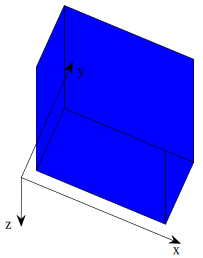
\includegraphics[clip]{WR}
    \caption{Guida rettangolare con propagazione dei campi lungo $\mathbf{\hat{z}}$}
    \label{fig:WR}
\end{figure}

\par La potenza che fluisce in guida \`e data dal flusso del vettore di Poynting dei campi modali \eqref{eqn:ModalFields} sulla superficie della sezione trasversale. Vengono scelti dei fattori di ampiezza $A_{mn}^{e,h}$ per le funzioni modali in modo da effettuare la seguente normalizzazione in potenza:
\begin{align}
P_{mn}^{e} = \frac{1}{2} \ \Re \left\{ \ \iint_A \left ( E_{xmn} H_{ymn}^{*} - E_{ymn} H_{xmn}^{*} \right ) dA \right\} = \frac{1}{2} \left [ |a_{mn}^{e}|^2 - |b_{mn}^{e}|^2 \right ] k_{mn}^{e} \omega \epsilon \notag \\
P_{mn}^{h} = \frac{1}{2} \ \Re \left\{ \ \iint_A \left ( E_{xmn} H_{ymn}^* - E_{ymn} H_{xmn}^* \right ) dA \right\} = \frac{1}{2} \left [ |a_{mn}^{h}|^2 - |b_{mn}^{h}|^2 \right ] k_{mn}^{h} \omega \mu
\end{align} dove $A$ \`e l'area della sezione.

\par Ogni segmento di guida avr\`a  le rispettive ampiezze dei coefficienti modali ${a}_{mn}^{e,h}$ e ${b}_{mn}^{e,h}$, incognite del problema della giunzione.  Per valutare l'entit\`a dell'accoppiamento tra modi di un segmento e l'altro della giunzione, si dovranno proiettare i campi di ciascuna regione nel medesimo spazio di funzioni, operazione senza la quale non potremmo confrontarli, e quindi verificare le condizioni al contorno. Come vedremo nel paragrafo \ref{SectionGradino}, nell'analisi del gradino, il \textit{set} di funzioni che semplifica la trattazione \`e dato dalle configurazioni modali di uno dei due segmenti giunti, a seconda della continuit\`a da imporre.

%%%%%%%%%%%%%%%%%%%%%%%%%%%%%
% GRADINO
\subsection{Il problema del gradino} \label{SectionGradino}

\par Vediamo come sia possibile applicare le condizioni al contorno al problema del gradino illustrato in figura \ref{fig:gradino}. Vi \`e rappresentato il problema del \textit{boundary enlargement}, per il quale la direzione $\mathbf{\hat{z}}$ di progressione delle onde vede susseguirsi un segmento di sezione $A_1$ e uno di sezione maggiore $A_2$.

\begin{figure}[hpt]
    \centering
    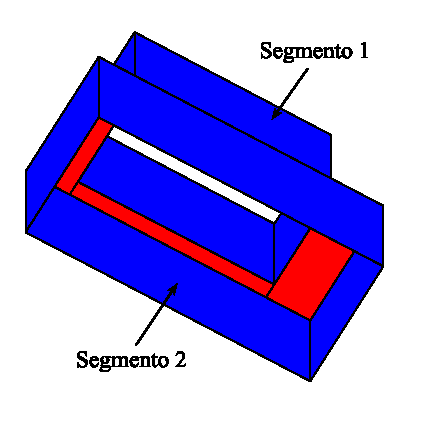
\includegraphics[clip, angle=0]{gradino}
    \caption{Struttura di una giunzione a gradino}
    \label{fig:gradino}
\end{figure}

\par Prima di procedere con l'imposizione della continuit\`a delle componenti tangenziali all'interfaccia, \`e necessario che le funzioni modali abbiano un medesimo riferimento cartesiano. Questo si ottiene con la semplice traslazione spaziale delle funzioni modali di uno o di entrambi i segmenti.

\par La continuit\`a dei campi modali \eqref{eqn:ModalFields} si riflette nella scelta delle funzioni di proiezione del campo: la possibilit\`a di annullare il campo elettrico trasverso su una porzione della superficie $A_2$, quella in corrispondenza di conduttore elettrico perfetto\footnote{Vale la condizione $\mathbf{E} \times \mathbf{\hat{z}} = 0$.\vspace*{3pt}} (p.e.c.) di giunzione tra i due segmenti data dalla differenza tra le aree $A_2$ e $A_1$, ci induce a proiettare i campi elettrici dei due segmenti nello spazio dei modi che costituiscono la base di espansione del campo nel segmento di guida 2; i campi magnetici trasversi vengono invece proiettati nello spazio dei modi del segmento 1:
\begin{align}
&\left.\mathbf{H}_t^{(2)} \right|_{A_1} = \left.\mathbf{H}_t^{(1)} \right|_{A_1} \notag \\
&\left.\mathbf{E}_t^{(2)} \right|_{A_2} = \left.\mathbf{E}_t^{(1)} \right|_{A_2}
\label{eq:continuity}
\end{align}
\par La proiezione dei campi trasversi dal loro spazio di espansione ad un altro viene fatta mediante il prodotto interno\footnote{Operazione definita entro spazi hilbertiani completi come quello delle configurazioni modali.}
\begin{align}
\langle \mathbf{V}_{ij} , \mathbf{W}_{kl} \rangle = \iint_A \mathbf{V}_{ij} \cdot \mathbf{W}_{kl} dA
\end{align} dove $\mathbf{V}_{ij}$ sono i modi da proiettare sullo spazio di arrivo dato dai modi $\mathbf{W}_{kl}$, e $A$ \`e il dominio di proiezione. Si ottengono quindi degli integrali di accoppiamento detti anche ``integrali di \textit{matching}'' in grado di definire per esempio, per un modo $\mathrm{TE}_{mn}$ progressivo con intensit\`a ${a_{mn}^{h}}^{(1)}$ nel segmento 1, quanta potenza viene trasferita a tutti i modi $\mathrm{TE}_{kl}$ e $\mathrm{TM}_{kl}$ progressivi ${b_{kl}^{e,h}}^{(2)}$ nel segmento 2. Questa caratteristica denota l'aspetto ``\textit{full-wave}'' del MM, in quanto vengono inclusi gli effetti di tutti i modi superiori alla discontinuit\`a, bench\'e essi possano essere evanescenti in entrambi i segmenti di guida. Si noti che i prodotti interni da calcolare sono risolvibili analiticamente come integrali curvilinei sui lati della sezione di riferimento, essendo le funzioni modali composte da funzioni trigonometriche \eqref{eq:ModeShapes} di facile integrazione. Inoltre, per una pi\`u semplice proiezione delle funzioni modali del segmento con sezione minore su quella di sezione maggiore, $A_2$ deve essere tale da comprendere interamente $A_1$, riducendo cos\`i l`integrale di \textit{matching} per la continuit\`a del campo elettrico all'area $A_2$ di riferimento e non ad un'area maggiore.
\par Data una frequenza di eccitazione della struttura, \`e possibile definire un sistema risolvente nelle incognite $a_{ij}^{e,h}$ e $b_{kl}^{e,h}$. Tale sistema, riscritto in forma matriciale, dovr\`a contenere un numero finito di incognite e quindi, per poter analizzare il problema, \`e necessario limitare il numero di modi utilizzati. Inoltre, l'analisi assistita da calcolatore \`e tale per cui la precisione a disposizione diverr\`a confrontabile con l'ampiezza dei modi superiori via via che se ne aumenter\`a l'ordine, troncando implicitamente la somma di modi. \`E comunque possibile definire un limite inferiore al numero di modi utilizzati, intrinseco alla tipologia di struttura guidante e dipendente dai parametri geometrici dei segmenti\footnote{Per esempio vale, per la guida rettangolare, la relazione $N_{modi} \geq \frac{10 \cdot \sqrt{a \cdot b}}{\lambda}$.}, per cui la potenza espansa numericamente converge a quella totale (corrispondente a quella all'espansione non troncata) entro una percentuale soddisfacente, tipicamente superiore a 99\%.
\par Il sistema risolvente del gradino \`e riconducibile, mediante operazioni algebriche, ad una matrice di \textit{scattering} $2 \times 2$, $\mathbb{S}_\mathrm{Gradino}$, della forma:
\begin{align}
\left[\begin{matrix} {b}_1 \\ {b}_2 \end{matrix}\right] &= \Big[ \mathbb{S}_\mathrm{Gradino} \Big] \left[\begin{matrix} {a}_1 \\ {a}_2 \end{matrix}\right] = \left[ \begin{matrix} \mathbb{S}_{11} & \mathbb{S}_{12} \\ \mathbb{S}_{21} & \mathbb{S}_{22} \end{matrix} \right] \left[\begin{matrix} {a}_1 \\ {a}_2 \end{matrix}\right]
\label{SmatrixGradino}
\end{align} dove ${a}_1$, ${b}_1$, ${a}_2$ e ${b}_2$ sono vettori colonna dei i modi considerati opportunamente ordinati. Si noti che la matrice $\mathbb{S}_\mathrm{Gradino}$ tiene conto della sola discontinuit\`a all'interfaccia tra i due segmenti. Per ottenere la matrice di \textit{scattering} vista dalle porte esterne del gradino in figura \ref{fig:gradino}, \`e necessario includere gli sfasamenti dei campi modali dovuti alle lunghezze dei segmenti. Quest'operazione viene fatta moltiplicando opportunamente gli elementi della matrice $\mathbb{S}_\mathrm{Gradino}$ con una matrice di \textit{delay}, matrice dei ritardi di fase di ciascun modo. Il problema della cascata di gradini si basa sull'unione delle matrici di \textit{scattering} di ciascuna giunzione, considerando gli sfasamenti dei campi modali dovuti ai tratti di linea che uniscono gradini consecutivi. Il gradino in configurazione \textit{boundary reduction} ha la medesima risposta elettromagnetica del \textit{boundary enlargement}. Avendo, da un punto di vista circuitale, scambiato le porte di ingresso e di uscita, \`e sufficiente trattare uno dei due casi per risolverli entrambi, ricombinando opportunamente gli elementi della matrice di \textit{scattering}.

%%%%%%%%%%%%%%%%%%%%%%%%%%%%%
% N to 1
\subsection{Il problema della giunzione N a 1} \label{SectionNto1}

\par L'N-forcazione si risolve in modo analogo al gradino. La differenza sostanziale sta nelle condizioni al contorno. Indicando come regione (1) quella degli N segmenti e come regione (2) quella del segmento che congiunge gli N segmenti, la continuit\`a delle componenti tangenziali si ottiene dalle seguenti relazioni: 
\begin{align}
&\left.\mathbf{H}_t^{(2)} \right|_{{A_1}^{[i]}} = \left.{\mathbf{H}_t^{(1)}}^{[i]} \right|_{{A_1}^{[i]}}  \ , \ \ \ \ i = \mathrm{1 \dots N} \notag \\
&\left.\mathbf{E}_t^{(2)} \right|_{A_2} = \sum_{i=1}^{\mathrm{N}} \left.{\mathbf{E}_t^{(1)}}^{[i]} \right|_{A_2}
\label{eq:continuityNto1}
\end{align} Vale il principio di sovrapposizione degli effetti e si pu\`o quindi dedurre la matrice del problema risolvente di tale giunzione dai contributi di ogni singolo gradino che la costituisce. I contributi congiunti tra gli N segmenti posti dallo stesso lato nascono dalla costruzione della matrice di \textit{scattering}. Si ottiene quindi una matrice di \textit{scattering} $\mathbb{S}_{\mathrm{N-forcazione}}$ che descrive il comportamento dell'interfaccia di giunzione, matrice $\mathrm{(N+1) \times (N+1)}$ della forma:
\begin{align}
\Big[ \mathbb{S}_{\mathrm{N-forcazione}} \Big] = \left[ \begin{matrix}
\mathbb{S}_{1,1} & \mathbb{S}_{1,2} & & \cdots & & \mathbb{S}_{1,N+1} \\
\mathbb{S}_{2,1} & \mathbb{S}_{2,2} & & \cdots & & \mathbb{S}_{1,N+1} \\
\vdots & \vdots & & \ddots & & \vdots \\
\mathbb{S}_{N+1,1} & \mathbb{S}_{N+1,2} & & \cdots & & \mathbb{S}_{N+1,N+1}
\end{matrix} \right] \label{SmatrixNto1}
\end{align} Come lo era per il singolo gradino, la matrice di \textit{scattering} alle porte esterne delle giunzioni si ricava con gli opportuni sfasamenti corrispondenti alle lunghezze dei segmenti.

\begin{figure}[hpt]
\centering
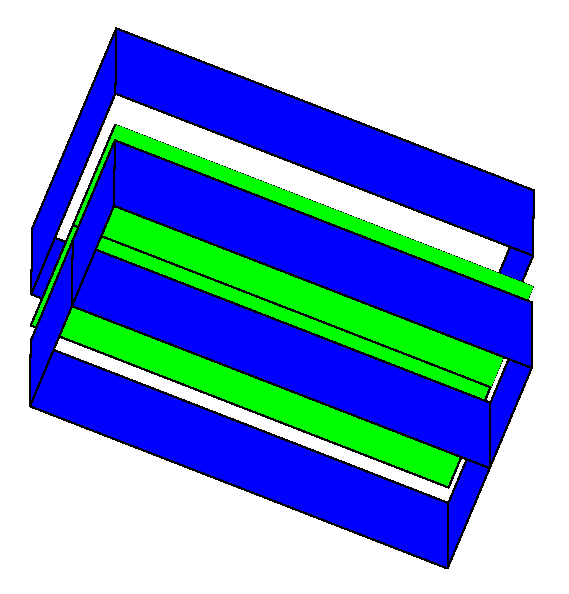
\includegraphics[scale=0.8]{bofNN}
\caption{Biforcazione nel piano E.}
\label{fig:bofNN}
\end{figure}

%%%%%%%%%%%%%%%%%%%%%%%%%%%%%
% COMPUTATIONS
\subsection{Implementazione numerica} \label{SectionImplNum}

\par Da un punto di vista computazionale, la teoria del MM presentata nei precedenti paragrafi \ref{SectionFormAnal}-\ref{SectionNto1} pu\`o essere riassunta nelle seguenti operazioni:
\begin{enumerate} \label{enum:passi}
\item esprimere il campo elettromagnetico trasverso in ogni segmento di guida come somma di funzioni modali,
\item applicare la continuit\`a delle componenti tangenziali del campo,
\item proiettare i modi di espansione del campo elettrico sulle funzioni modali corrispondenti alla guida di sezione pi\`u ampia e i modi  del campo magnetico sulle funzioni modali corrispondenti alla guide di sezioni pi\`u strette, deducendo gli integrali di \textit{matching} e procedendo con la loro soluzione analitica in forma chiusa,
\item costruire un sistema risolvente in forma matriciale, le cui incognite sono le onde incidenti $\mathbf{\mathit{a}}$ e riflesse $\mathbf{\mathit{b}}$ sulla discontinuit\`a, 
\item ricondurre il sistema risolvente ad una matrice di \textit{scattering}, della forma \eqref{SmatrixGradino} per un gradino e \eqref{SmatrixNto1} per la giunzione N a 1. Quest'ultima viene schematizzata in figura \ref{fig:SNto1} con un blocco di N+1 porte.\label{Algoritmo}
\end{enumerate}

\begin{figure}[hpt]
\centering
\includegraphics[scale=0.8]{SNto1}
\caption{Blocco schematico di una generica giunzione N a 1.}
\label{fig:SNto1}
\end{figure}

\par Sono state realizzate delle funzioni Matlab che implementano le 5 fasi dell'algoritmo precedentemente elencato. In particolare, le funzioni ``\textit{\textsf{Multistep}}'' e ``\textit{\textsf{Nto1Junction}}'' costituiscono il cuore del programma: ricevendo in ingresso parametri relativi alla geometria della struttura, quali le lunghezze d'onda di \textit{cut-off} dei modi che espandono il campo in guida e le aree di affacciamento ad una giunzione, queste funzioni restituiscono per la frequenza di lavoro richiesta le rispettive matrici di \textit{scattering}, la prima di una cascata di gradini e la seconda di una giunzione N a 1. Una funzione chiamante per la soluzione di un dispositivo composto da simili blocchi si occuper\`a quindi di analizzare i dati geometrici e topologici dei segmenti giunti per poi chiamare le funzioni \textit{\textsf{Multistep}} e \textit{\textsf{Nto1Junction}} su un'insieme di righe spettrali, in modo da ricavare il comportamento del dispositivo su di una banda pi\`u ampia.

%%%%%%%%%%%%%%%%%%%%%%%%%%%%% BIFORCAZIONE
\subsubsection*{Analisi di una biforcazione}\label{sec:bifocazione}

\begin{figure}[hpt]
\centering
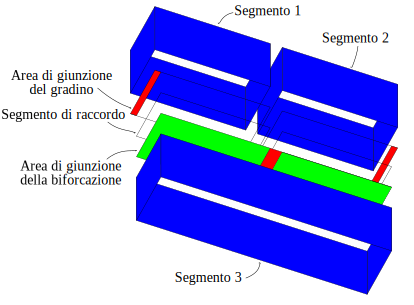
\includegraphics[clip]{bofNNh}
\caption{Biforcazione nel piano H con incompleta sovrapposizione delle guide.}
\label{fig:bofNNh}
\end{figure}

\par Procediamo con l'analisi della struttura illustrata in figura \ref{fig:bofNNh}. Trattasi di una biforcazione per la quale la guida 3 di sezione maggiore non include completamente le sezioni delle altre guide 1 e 2. Per poter valutare gli integrali di \textit{matching}, viene inserito in prossimit\`a della superficie di giunzione dei segmenti di guida di lunghezza nulla tali per cui le sezioni si sovrappongano correttamente. Questi segmenti fittizi serviranno da raccordo tra la giunzione e i segmenti 1 e 2.

\par Le guide 1 e 2 sono delle WR75 (0,75''$\times$0,375'') e il lato \textsf{a} della terza guida \`e leggermente pi\`u lungo del doppio delle altre. Vi \`e quindi uno scostamento maggiore delle guide 1 e 2 rispetto all'asse longitudinale della guida 3 per avere la non totale sovrapposizione delle aree di \textit{matching}.

\par Risolvere l'intera struttura significa determinare la matrice di \textit{scattering} $3 \times 3$ vista dalle onde modali incidenti alle porte esterne dei segmenti 1, 2 e 3. Per calcolarla abbiamo deciso di scomporre il problema in quattro sotto-problemi: la struttura pu\`o essere vista come composta da tre strutture guidanti di soli gradini ed una giunzione di raccordo  come viene illustrato nello schema a blocchi risolutivo di figura \ref{fig:SchemabofNNh}. 

\begin{figure}[hpt]
\centering
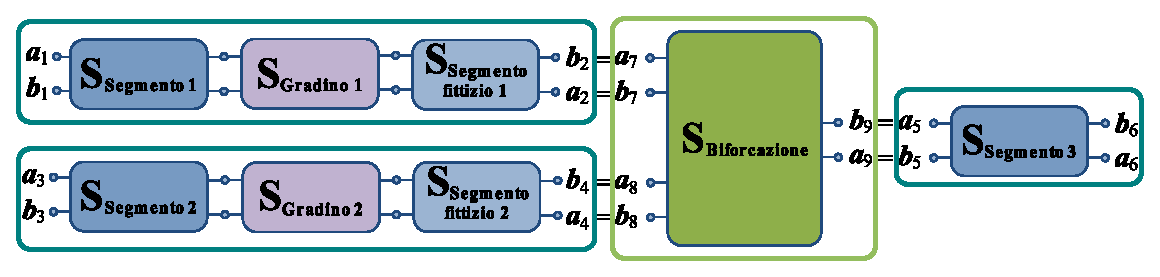
\includegraphics[scale=0.8]{SchemabofNNh1}
\caption{Schema a blocchi della biforcazione da analizzare.}
\label{fig:SchemabofNNh}
\end{figure}

\par Con questo schema a blocchi abbiamo stabilito una numerazione globale per le porte principali del problema: due porte per ogni cascata di gradini e per il tronco di linea dato dal segmento 3, tre porte per la giunzione ``2 a 1''. Le porte esterne della struttura sono le 1, 3 e 6.

\par Una volte ricavate le matrici di \textit{scattering} di ciascun blocco, \`e necessario assemblarle. Supponiamo di avere N blocchi tra cascate di gradini e giunzioni, le N rispettive matrici possono essere raggruppate, disponendole diagonalmente in una matrice pi\`u ampia, la \textit{Generalized Scattering Matrix} (GSM):
\begin{align}
\mathrm{GSM} = \left[ \begin{matrix}
\left[\mathbb{S}_1\right]&&&&\\
&\left[\mathbb{S}_2\right]&&&\\
&&\ddots&&\\
&&&&\left[\mathbb{S}_\mathrm{N}\right]
\end{matrix} \right] \label{GSM}
\end{align} Nel caso nostro otterremo una diagonale composta dalle tre matrici $2 \times 2$ dei gradini e dalla matrice $3 \times 3$ della giunzione 2 a 1. L'algoritmo di condensazione di GSM presentato in \cite{SSelleri} \`e stato implementato nel programma ``\textsf{CondenseGSM}''. Per ridurre la GSM alle porte esterne si procede eguagliando i campi modali incogniti relativi a due blocchi connessi, ad esempio per il blocco relativo al segmento 1 e la biforcazione, collegati tramite le porte 2 e 7. Si ottengono quindi delle equazioni che mettano in relazione le onde incidenti alle porte collegate ad atre porte della struttura. \`E quindi possibile riscrivere l'intero sistema risolvente eliminando le porte appena collegate. Procedendo iterativamente, si giunge ad un'equazione matriciale relativa alle sole porte esterne del sistema.

\par Un'operazione di notevole importanza \`e quella della rinormalizzazione delle GSM. In effetti, le espressioni analitiche della continuit\`a dei campi \eqref{eq:continuity} e \eqref{eq:continuityNto1} sono tali da conferire una dipendenza spettrale $jk_{mn}$ alle ampiezze modali di un segmento. La funzione ``\textsf{Renormalize}'' viene applicata ad una matrice di \textit{scattering} condensata, riferendola alle porte esterne e quindi ai rispettivi numeri d'onda $k_{mn}$, strettamente legati alla sezione del segmento corrispondente. Si ottengono cos\`i coefficienti di \textit{scattering} normalizzati.

\par Si noti che la cascata di gradini stessa pu\`o essere vista come un sistema di blocchi connessi, come illustrato in figura \ref{fig:SchemabofNNh}, e la funzione \textsf{Multistep} potrebbe essere realizzata con operazioni di condensazione e rinormalizzazione agli estremi.

\par La simulazione della struttura \`e stata condotta sia col metodo del MM implementato che con il simulatore commerciale dell'Ansoft, HFSS, il quale implementa il FEM. In figura \ref{fig:bofNNhResults} vi sono illustrati i risulati delle simulazioni, avendo eseguito per entrambe uno \textit{sweep} in frequenza da 10 a 25 GHz e rappresentato, considerando il modo TE$_{10}$ di eccitazione alla porta 1, il modo TE$_{10}$ riflesso alla medesima porta ($\mathbb{S}{11}_{{h10}_{h10}}$), i modi TE$_{10}$ trasmessi alle porte 2 e 3 ($\mathbb{S}{21}_{{h10}_{h10}}$ e $\mathbb{S}{31}_{{h10}_{h10}}$) ed infine i modi di ordine superiore TE$_{20}$, TE$_{30}$, TE$_{40}$ e TE$_{50}$ alla porta 3 ($\mathbb{S}{31}_{{h20}_{h10}}$, $\mathbb{S}{31}_{{h30}_{h10}}$, $\mathbb{S}{31}_{{h40}_{h10}}$ e $\mathbb{S}{31}_{{h50}_{h10}}$). Per il MM sono stati impiegati 16 modi di espansione. Il numero di punti frequenziali \`e di 61 per entrambi i metodi. I tempi di simulazione, sulla medesima macchina, sono stati del minuto per il MM e dell'ordine dell'ora per il FEM.

\begin{figure}[hpt]
\centering
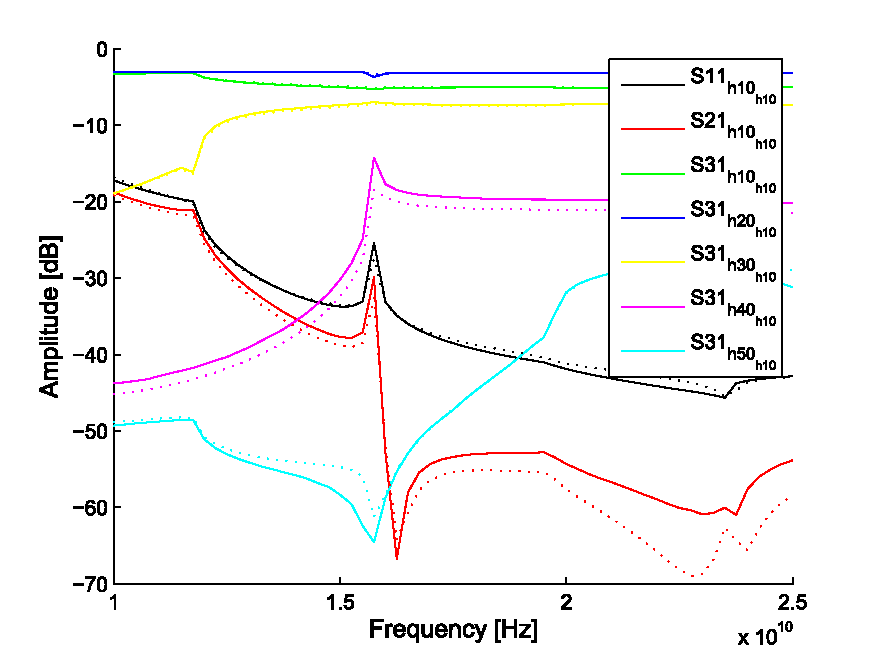
\includegraphics[scale=1]{bofNNhResults}
\caption{Risultati a confronto tra quelli ottenuti col MM implementato (---) e quelli ottenuti col simulatore HFSS ($\ldots$) per la biforcazione di figura \ref{fig:bofNNh}.}
\label{fig:bofNNhResults}
\end{figure}

\par Il modo fondamentale nelle WR75 nasce intorno ai 7,78 GHz, frequenza alla quale nella guida 3 il modo TE$_{20}$ si trova in condizioni di propagarsi. Fino alla frequenza di attivazione del modo TE$_{30}$ nella guida 3, intorno ai 11,8 GHz, la potenza del segnale in banda unimodale iniettato nella guida 1 viene conteso tra i modi TE$_{10}$ e TE$_{20}$ nella guida 3. Per ragioni che possiamo intuitivamente ricondurre alla distribuzione spaziale dei campi modali, il modo TE$_{30}$ assorbe prevalentemente la potenza precedentemente destinata al modo TE$_{10}$, lasciando inalterato il modo TE$_{20}$ a -3 dB. Il modo TE$_{40}$, con frequenza critica intorno ai 15,7 GHz disturba lievemente il TE$_{20}$ in guida 3 ed \`e tale da assorbire maggior potenza dal modo TE$_{20}$ che si innesca nella guida 2 alla medesima frequenza (l'$\mathbb{S}{21}_{{h10}_{h10}}$ si riduce drasticamente cedendo potenza all'$\mathbb{S}{21}_{{h20}_{h10}}$ che a sua volta la cede all'$\mathbb{S}{31}_{{h40}_{h10}}$).

\par \`E interessante vedere che gli andamenti dei grafici sono simili, verificando la corretta implementazione della tecnica. La possibilit\`a di applicare il metodo a strutture di complessit\`a maggiore suscita un notevole interesse: la variazione dei parametri geometrici per rientrare entro delle specifiche di progetto di un certo dispositivo si esegue in tempi notevolmente ridotti, velocizzando il progetto di una tale struttura.

%%%%%%%%%%%%%%%%%%%%%%%%%%%%%%%%%%%%%%%%%%%%%%%%%%%%%%%%%%%%%%%%%%%%%%%%%%%%%%%% % HILDEBRAND'S COUPLER
\section{L'accoppiatore direzionale di Hildebrand}\label{BigSecCoupler}

\par L. T. Hildebrand descrive in \cite{LTHildebrand} l'analisi MM di un accoppiatore direzionale di tipo Riblet. I grafici che presenta, derivati da una sua implementazione del MM, hanno prodotto buone similitudini con quelli che ha ottenuto da una simulazione con HFSS (\cite{LTHildebrand}-\textit{III. Results}). Ci siamo riferiti a questi grafici per verificare i risultati ottenuti con l'implementazione discussa nel precedente paragrafo \ref{BigSecMM}.

%%%%%%%%%%%%%%%%%%%%%%%%%%%%%
% STRUTTURA
\subsection{Struttura}

\begin{figure}[hpt]
\centering
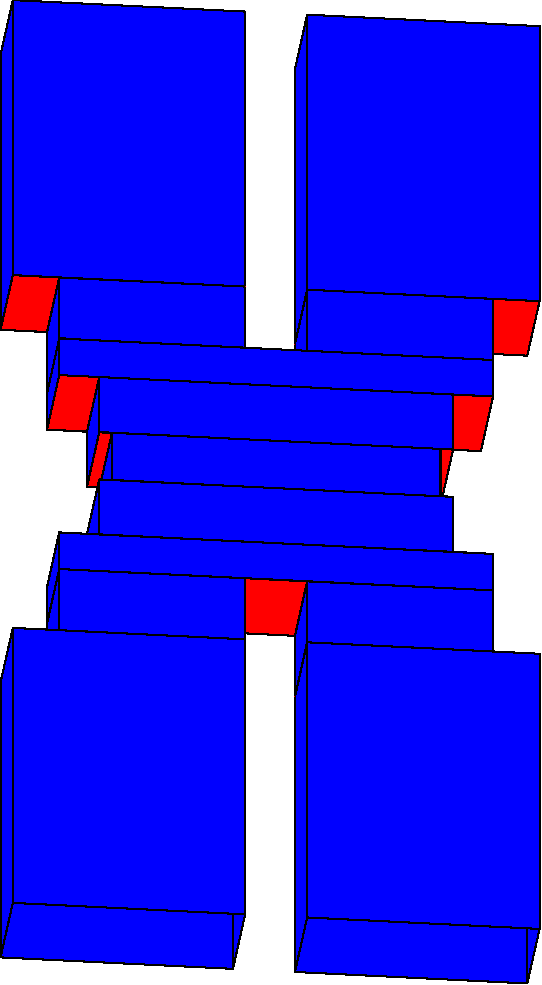
\includegraphics[scale=0.5, angle=90]{Hildebrand}
\caption{Struttura dell'accoppiatore direzionale di Hildebrand.}
\label{fig:Hildebrand}
\end{figure}

\par Analizziamo la struttura dell'accoppiatore direzionale in figura \ref{fig:Hildebrand}. Trattasi di una giunzione ibrida di tipo Riblet \cite{HJRiblet}, ossia una giunzione costituita da due segmenti di guida uniti nel piano H da un'apertura dimensionata in modo da presentare, ad una determinata frequenza, le seguenti caratteristiche:
\begin{itemize}
\item dal lato di iniezione del segnale non vi \`e alcun campo riflesso e queste prime due porte vengono chiamate ``porta d'ingresso'' e ``porta isolata'',
\item dal lato opposto fuoriesce tutto il campo iniettato, diviso tra la ``porta di trasmissione'' appartenente allo stesso segmento di guida della porta d'ingresso e la ``porta accoppiata'' dell'altro segmento,
\item la caratteristica ``ibrida'' \`e legata alla divisione equa della potenza tra le porte di uscita, ossia -3dB rispetto alla porta di ingresso per entrambe,
\item vi \`e una fase relativa tra i segnali di uscita di 90�.
\end{itemize}
Le precedenti caratteristiche corrispondono ad un'ibrido ideale ed \`e necessario poter esprimere le prestazioni di un accoppiatore direzionale reale. Si introducono quindi i seguenti parametri tratti da \cite{SteerTrew}:
\begin{itemize}
\item ``fattore di accoppiamento'': rapporto tra la potenza in ingresso e quella in uscita alla porta accoppiata,
\item ``direttivit\`a'': rapporto tra la potenza in uscita alla porta accoppiata e quella che giunge alla porta isolata,
\item ``fattore di isolamento'': rapporto tra la potenza in ingresso e quella che giunge alla porta isolata.
\end{itemize}

\par L'accoppiatore di Hildebrand \`e una versione modificata della ``\textit{Short-Slot Hybrid Junction}'' di H. J. Riblet illustrata in figura \ref{fig:Riblet}. La banda\footnote{Per banda si intende lo spettro per il quale un dispositivo preserva, entro certe tolleranze, le caratteristiche elettromagnetiche specificate.} di quest'ultimo dispositivo \`e particolarmente stretta e buone prestazioni a larga banda si ottengono caricando capacitivamente (ad esempio con una vite micrometrica) la regione di accoppiamento. L'allargamento della banda dell'ibrido di Hildebrand si ottiene realizzando una regione di accoppiamento con una cascata di gradini, assicurando cos\`i un addattamento di impedenza graduale. Un tale dispositivo presenta numerosi vantaggi rispetto all'ibrido di Riblet caricato capacitivamente, nonostante non si raggiungano le medesime prestazioni. La semplicit\`a realizzativa e di impiego fa della giunzione di Hildebrand una buona alternativa nelle applicazioni a banda relativamente stretta.

\begin{figure}[hpt]
\begin{minipage}[b]{0.5\linewidth} % A minipage that covers half the page
\centering
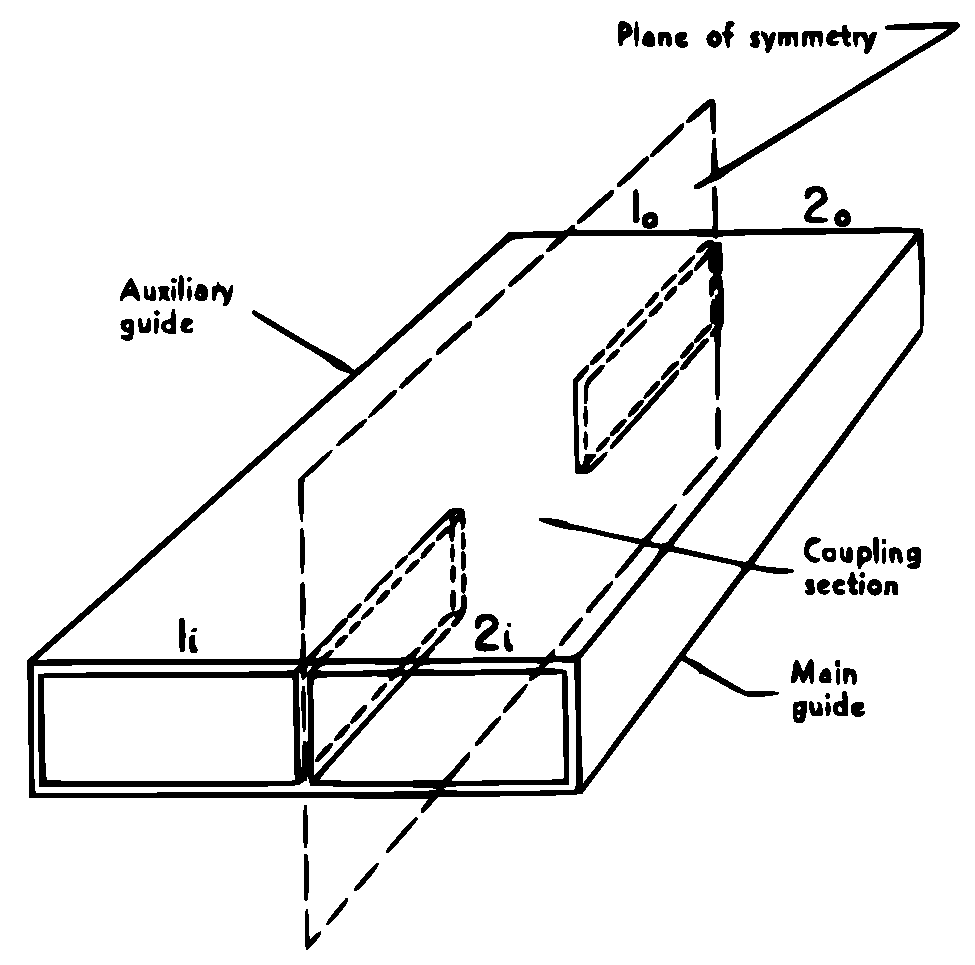
\includegraphics[scale=0.3]{Riblet}
\caption{Struttura dell'accoppiatore direzionale di Riblet. \cite{HJRiblet}}
\label{fig:Riblet}
\end{minipage}
\hspace{0.1cm} % To get a little bit of space between the figures
\begin{minipage}[b]{0.5\linewidth}
\centering
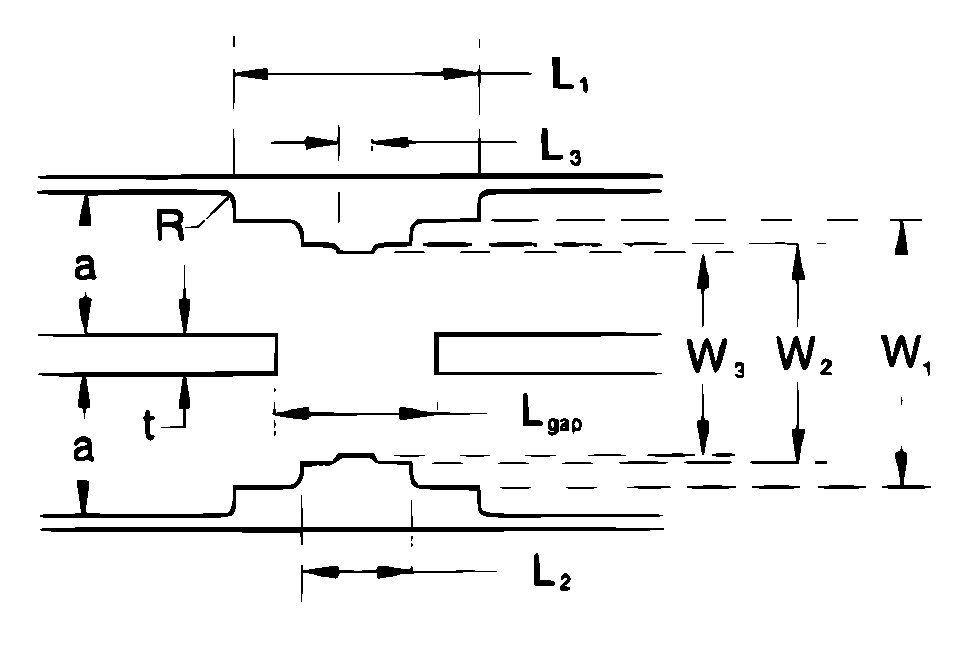
\includegraphics[scale=0.5]{HildPaperStruct}
\caption{Geometria dell'accoppiatore direzionale di Hildebrand. \cite{LTHildebrand}}
\label{fig:HildPaperStruct}
\end{minipage}
\end{figure}

\par Le dimensioni dell'accoppiatore di Hildebrand, progettato per operare intorno ai 14 GHz, sono tali da raccordare delle guide WR75. Le dimensioni, in pollici, riportate in figura \ref{fig:HildPaperStruct} sono le seguenti: {a = 0.75'',} {b = 0.375'',} {t = 0.2'',} {R = 0.040'',} {L$_1$ = 1.282'',} {L$_2$ = 0.572'',} {L$_3$ = 0.172'',} {L$_{gap}$ = 0.838'',} {W$_1$ = 1.4'',} {W$_2$ = 1.142''} e {W$_3$ = 1.06''.} Nella nostra simulazione si considera nullo il raggio di curvatura R delle WR75, bench\'e potremmo facilmente includere questo parametro discretizzando la curvatura con una cascata di guide via via pi\`u strette e di lunghezza infinitesima rispetto al raggio.

%%%%%%%%%%%%%%%%%%%%%%%%%%%%%%%%%%%%%%%
\subsection{Schema di analisi}\label{SectionSchemaAnalisiHild}

\par L'accoppiatore di Hildebrand \`e complessivamente composto da 13 segmenti di guida disposti in 5 cascate di gradini e da 2 biforcazioni. In figura \ref{fig:HildebrandExploded} sono illustrati i componenti disgiunti della struttura.

\begin{figure}[hpt]
\centering
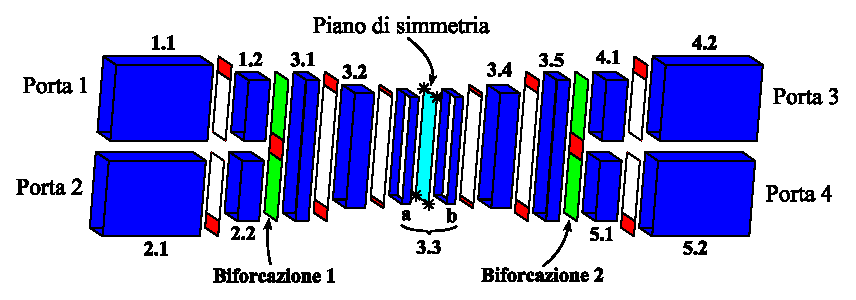
\includegraphics[scale=1, angle=0]{HildebrandExploded}
\caption{Struttura dettagliata dell'accoppiatore direzionale di Hildebrand con sezione nel piano trasversale di simmetria.}
\label{fig:HildebrandExploded}
\end{figure}

\par L'accoppiatore di Hildebrand gode di una simmetria interessante dal punto di vista computazionale: \`e possibile individuare un piano trasversale che divida in due parti uguali la struttura e, procedendo con la soluzione di una sola delle parti, ricondurre i risultati all'intera struttura. Tale piano \`e localizzato, come si pu\`o vedere in figura \ref{fig:HildebrandExploded} alla mezzeria del terzo segmento della cascata di gradini confinata entro le due aree di biforcazione. L'analisi si riduce quindi alla computazione delle matrici di \textit{scattering} dei gradini 1 (segmenti 1.1 e 1.2) e 2 (segmenti 2.1 e 2.2), di met\`a gradino 3 (segmenti 3.1, 3.2 e 3.3a) e della biforcazione 1. Si ottiene, analogamente a quanto fatto nel paragrafo \ref{sec:bifocazione}, quattro matrici di \textit{scattering}. Ottenuta la GSM relativa ai quattro blocchi, questa verr\`a condensata alle porte aperte dei segmenti 1.1, 2.1 e 3.3 nella seguente matrice $3 \times 3$:
\begin{align}
\mathbb{S}_\textrm{half} = \left[ \begin{matrix} \mathbb{S}_{11} & \mathbb{S}_{12} & \mathbb{S}_{13}  \\ \mathbb{S}_{21} & \mathbb{S}_{22} & \mathbb{S}_{23} \\ \mathbb{S}_{31} & \mathbb{S}_{32} & \mathbb{S}_{33} \end{matrix} \right]
\end{align}
Per aggiungere l'altra met\`a ai risultati ottenuti \`e sufficiente raddoppiare la matrice $\mathbb{S}_\textrm{half}$ e disporre le due matrici identiche in una nuova GSM, la quale avr\`a come porte associate le porte aperte dei segmenti 1.1, 2.1 e 3.3a per la prima sotto-matrice e le porte aperte dei segmenti 4.2, 5.2 e 3.3b per la seconda:
\begin{align}
\left[ \begin{matrix} \left[ \begin{matrix} b_\mathrm{1.1} \\ b_\mathrm{2.1} \\ b_\mathrm{3.3a} \end{matrix} \right] \\ \left[ \begin{matrix} b_\mathrm{4.2}\\ b_\mathrm{5.2} \\ b_\mathrm{3.3b} \end{matrix} \right] \end{matrix} \right] = \left[ \begin{matrix} \left[ \begin{matrix} \mathbb{S}_{11} & \mathbb{S}_{12} & \mathbb{S}_{13}  \\ \mathbb{S}_{21} & \mathbb{S}_{22} & \mathbb{S}_{23} \\ \mathbb{S}_{31} & \mathbb{S}_{32} & \mathbb{S}_{33} \end{matrix} \right] & \\
& \left[ \begin{matrix} \mathbb{S}_{11} & \mathbb{S}_{12} & \mathbb{S}_{13}  \\ \mathbb{S}_{21} & \mathbb{S}_{22} & \mathbb{S}_{23} \\ \mathbb{S}_{31} & \mathbb{S}_{32} & \mathbb{S}_{33} \end{matrix} \right] \end{matrix} \right] \left[ \begin{matrix} \left[ \begin{matrix} a_\mathrm{1.1} \\ a_\mathrm{2.1} \\ a_\mathrm{3.3a} \end{matrix} \right] \\ \left[ \begin{matrix} a_\mathrm{4.2}\\ a_\mathrm{5.2} \\ a_\mathrm{3.3b} \end{matrix} \right] \end{matrix} \right]
\label{newGSM}
\end{align}
Si procede quindi con la condensazione, le porte aperte dei segmenti 3.3a e 3.3b dovendo essere connesse. Si ottiene una matrice della forma:
\begin{align}
\left[ \begin{matrix}  b_\mathrm{1.1} \\ b_\mathrm{2.1} \\ b_\mathrm{4.2} \\ b_\mathrm{5.2} \end{matrix} \right] = \left[ \begin{matrix} \mathbb{S'}_{11} & \mathbb{S'}_{12} & \mathbb{S'}_{13} & \mathbb{S'}_{14} \\ 
\mathbb{S'}_{21} & \mathbb{S'}_{22} & \mathbb{S'}_{23} & \mathbb{S'}_{24} \\
\mathbb{S'}_{31} & \mathbb{S'}_{32} & \mathbb{S'}_{33} & \mathbb{S'}_{34} \\
\mathbb{S'}_{41} & \mathbb{S'}_{42} & \mathbb{S'}_{43} & \mathbb{S'}_{44} \end{matrix} \right] \left[ \begin{matrix} a_\mathrm{1.1} \\ a_\mathrm{2.1} \\ a_\mathrm{4.2} \\ a_\mathrm{5.2} \end{matrix} \right]
\label{lastGSM}
\end{align} che descrive il comportamento dell'accoppiatore direzionale di Hildebrand ad una determinata frequenza di eccitazione. I risultati verranno discussi nel paragrafo \ref{SectionRisultati}, confrontandoli con quelli ottenuti da Hildebrand.

\par Si noti che la computazione diretta della matrice di \textit{scattering} della struttura simmetrica 1 a N si ottiene con la ridisposizione temporanea dei segmenti, riconducendo tale giunzione ad una N a 1 identicamente simmetrica.

\par Questo metodo di analisi considerava la presenza di un'unica area di n-forcazione. \`E stata implementata, per estendere il codice precedentemente sviluppato, la possibilt\`a di analizzare una struttura composta da un numero maggiore di n-forcazioni e, percorrendone una alla volta, di risolvere il ``macroblocco'' composto dall'area di n-forcazione e delle strutture a gradini adiacenti. 

\begin{figure}[hpt]
\begin{minipage}[b]{0.5\linewidth} % A minipage that covers half the page
\centering
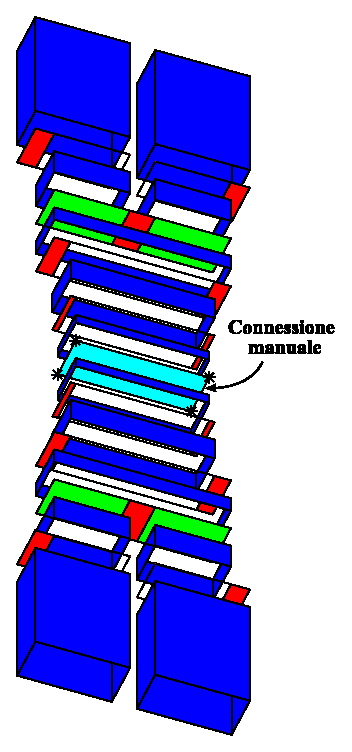
\includegraphics[width=5.2cm]{HildebrandExploded1}
\caption{Struttura dettagliata dell'accoppiatore direzionale di Hildebrand ottenuta con la dichiarazione esplicita di una connessione inter-macroblocchi.}
\label{fig:HildebrandExploded1}
\end{minipage}
\begin{minipage}[b]{0.5\linewidth}
\centering
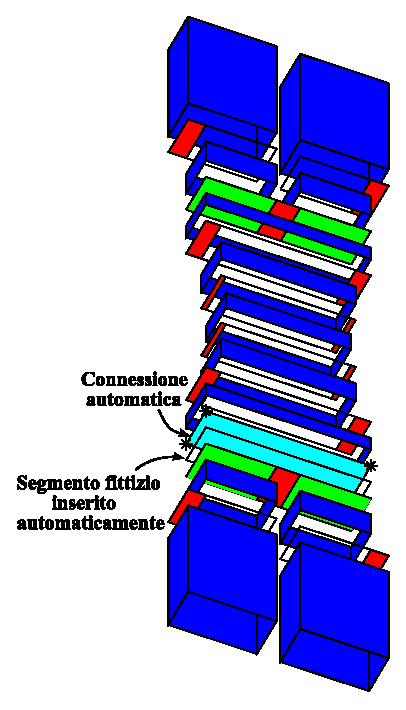
\includegraphics[width=6.5cm]{HildebrandExploded2}
\caption{Struttura dettagliata dell'accoppiatore direzionale di Hildebrand ottenuta con la separazione automatica delle biforcazioni.}
\label{fig:HildebrandExploded2}
\end{minipage}
\end{figure}

\`E possibile richiedere esplicitamente, come si pu\`o vedere in figura \ref{fig:HildebrandExploded1}, la connessione di macroblocchi per ottenere la matrice di \textit{scattering} dell'intero problema. Qualora alcuni macroblocchi dovessero presentare strutture a gradini condivise, vi \`e la possibilit\`a di inserire automaticamente un segmento di lunghezza nulla come viene illustrato in figura \ref{fig:HildebrandExploded2} e separare cos\`i i blocchi congiunti. Entrambe le configurazioni riconducono alla medesima matrice di \textit{scattering} \eqref{lastGSM}.

\par Ricapitolando, \`e possibile definire la seguente serie di passaggi risolutivi per un generico dispositivo composto da giunzioni trasversali\footnote{Il codice che \`e stato implementato risolve soltanto delle giunzioni per le quali la continuit\`a dei campi \`e associata alle loro componenti trasversali. Un gomito o una giunzione a T richiede l'aggiunta di un modulo risolvente che tratti le componenti longitudinali dei campi per eccitare modi che si possono propagare trasversalmente.\cite{SieveArndt}} quali gradini e n-forcazioni:
\begin{itemize}
\item controllare i dati in ingresso relativi allo \textit{sweep} in frequenza e quelli geometrici e topologici della struttura, 
\item procedere, per ogni frequenza richiesta, con la soluzione schematizzata nel diagramma di flusso di figura \ref{fig:FluxDiag},
\item presentare i dati elaborati.
\end{itemize}

\begin{figure}[hpt]
\centering
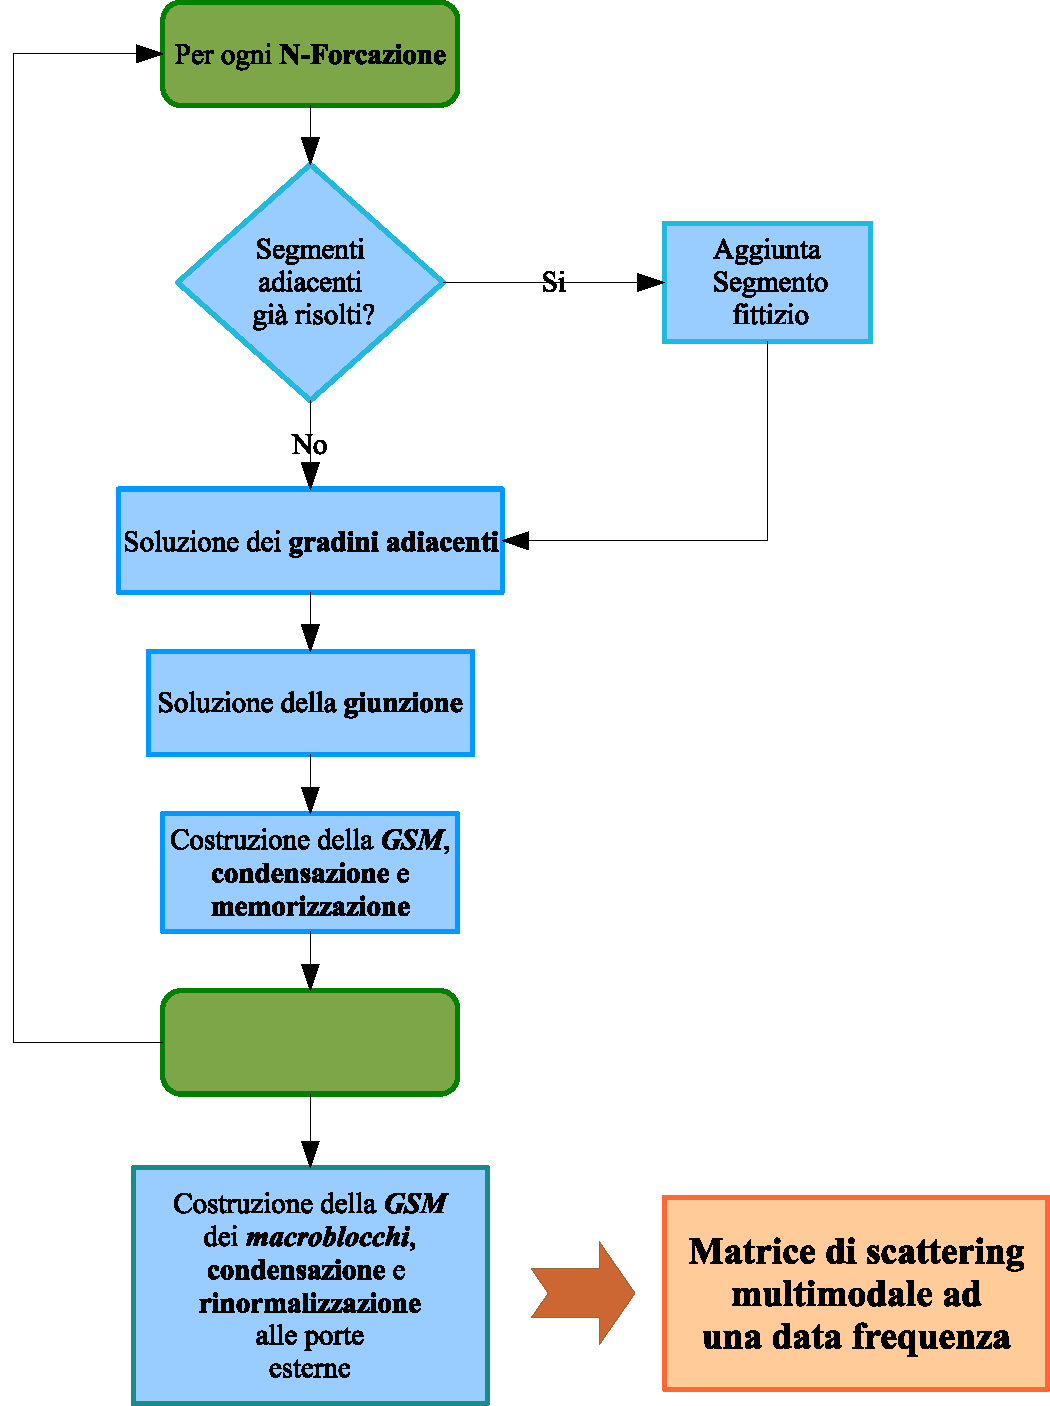
\includegraphics[width=14cm]{FlowDiag}
\caption{Diagramma di flusso del programma per la soluzione di un generico dispositivo.}
\label{fig:FluxDiag}
\end{figure}

\subsection{Risultati}\label{SectionRisultati}

\par Vediamo adesso i risultati ottenuti dalle simulazioni, identici per i tre metodi di analisi descritti nel precedente paragrafo \ref{SectionSchemaAnalisiHild}. Le simulazioni sono state eseguite considerando 13 modi di espansione su 51 punti frequenziali equidistanti nell'intervallo che va da 13 a 15 GHz. I coefficienti di diffusione illustrati sono corrispondenti al solo modo fondamentale. Le figure relative alle simulazioni di Hildebrand comprendono grafici di misure effettuate su un dispositivo dimensionato come in figura \ref{fig:HildPaperStruct}.

\begin{figure}[h!]
\begin{minipage}[b]{0.5\linewidth} % A minipage that covers half the page
\centering
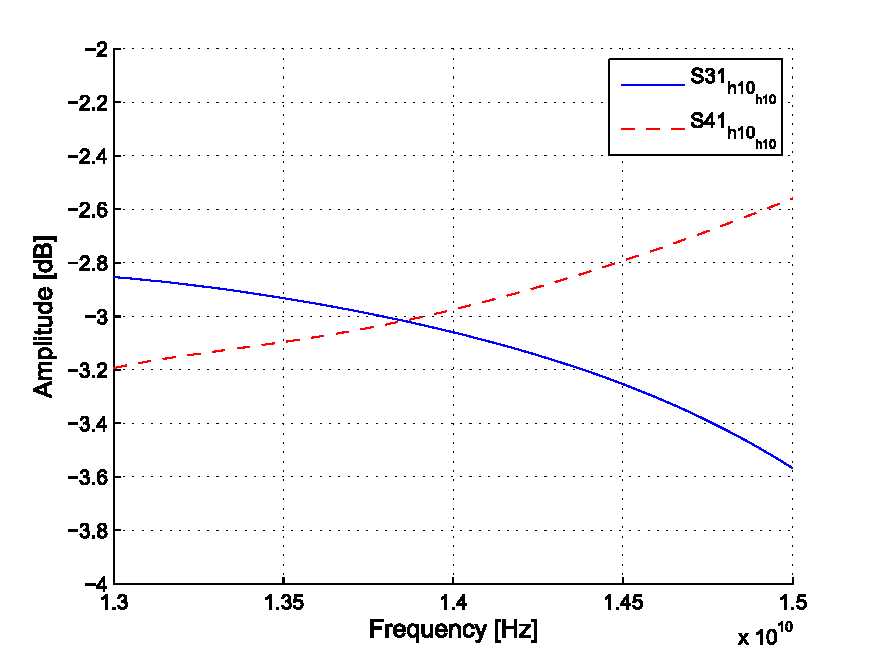
\includegraphics[width=7cm]{HybridResults}
\caption{Parametri di trasmissione.}
\label{fig:Trans}
\end{minipage}
\begin{minipage}[b]{0.5\linewidth}
\centering
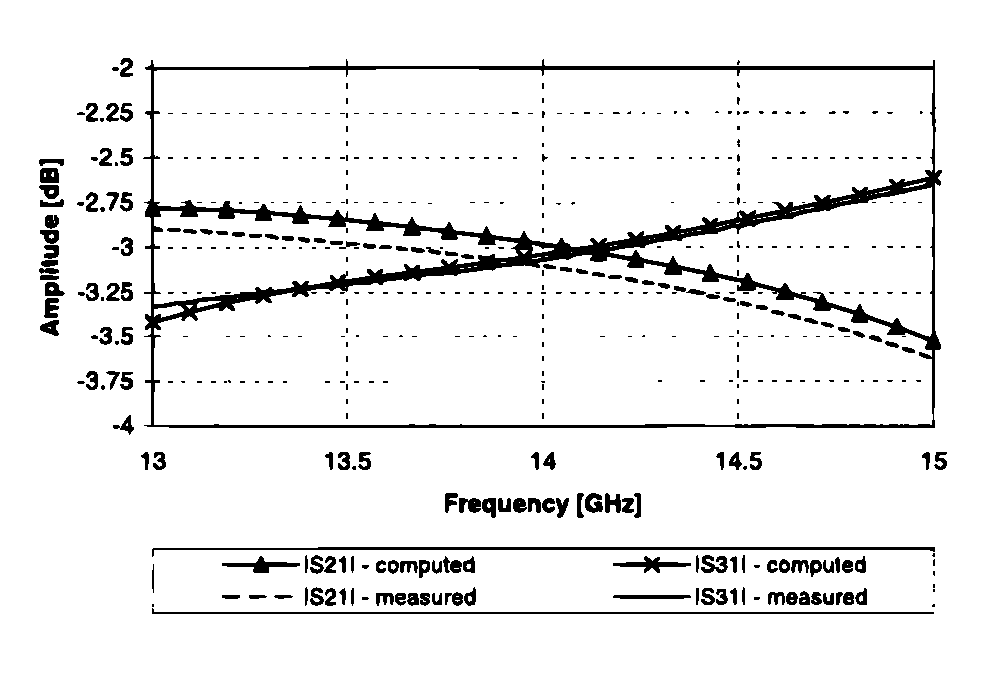
\includegraphics[width=7cm]{HildPaperTrans}
\caption{Parametri di trasmissione ottenuti da Hildebrand.}
\label{fig:TransH}
\end{minipage}
\end{figure}
\par Nelle figure \ref{fig:Trans} e \ref{fig:TransH} si illustrano i parametri di trasmissione che verificano la caratteristica ibrida dell'accoppiatore direzionale, nella prima quelli ottenuti dalla nostra simulazione e nella seconda quelli pubblicati da Hildebrand. La nostra simulazione presenta una frequenza di incrocio tra il coefficiente di trasmissione alla porta diretta ($\mathbb{S}{31}_{{h10}_{h10}}$, S21 per Hildebrand) e quello alla porta accoppiata ($\mathbb{S}{41}_{{h10}_{h10}}$, S31 per Hildebrand) di circa 13,8 GHz, frequenza alla quale la potenza viene divisa equamente entro le porte di uscita e che chiameremo ``frequenza centrale''. Tali parametri restano, nell'intervallo di frequenze considerato, entro $\pm$0.6 dB. La banda a -3dB $\pm$0.125 dB riduce l'intervallo di lavoro entro 13,35 e 14,25 GHz, implicando una banda relativa di soli 6.5\% rispetto ai 15\% ottenuti con un ibrido Riblet caricato capacitivamente.

\begin{figure}[h!]
\begin{minipage}[b]{0.5\linewidth} % A minipage that covers half the page
\centering
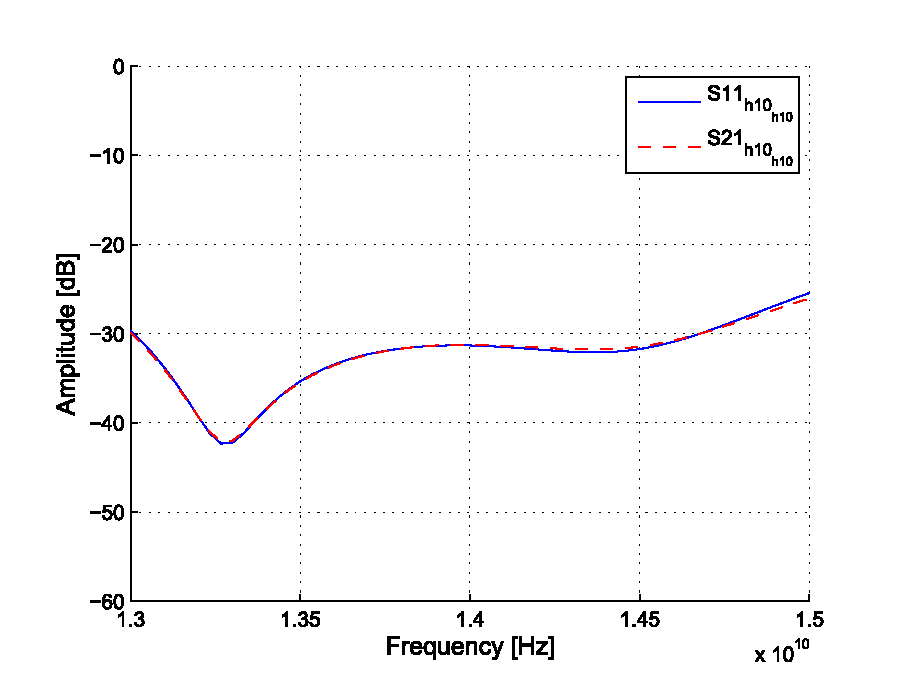
\includegraphics[width=7cm]{ReflectionCoeff}
\caption{Parametri di riflessione.}
\label{fig:Refl}
\end{minipage}
\hspace{0.1cm} % To get a little bit of space between the figures
\begin{minipage}[b]{0.5\linewidth}
\centering
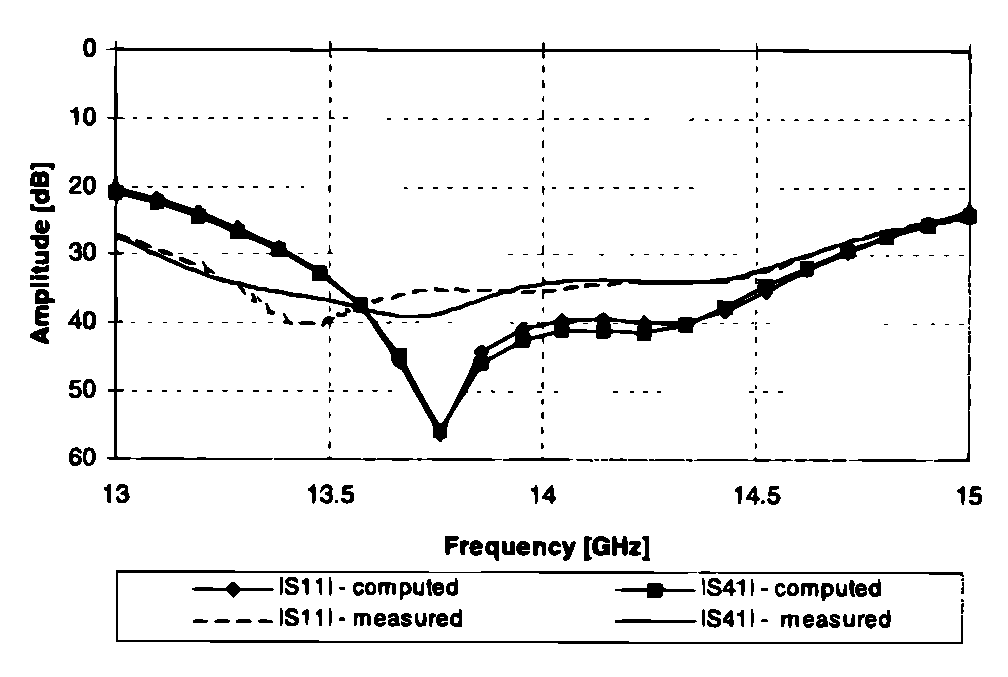
\includegraphics[width=7cm]{HildPaperRefl}
\caption{Parametri di riflessione ottenuti da Hildebrand.}
\label{fig:ReflH}
\end{minipage}
\end{figure}

\par Nelle figure \ref{fig:Refl} e \ref{fig:ReflH} vengono illustrati i parametri di riflessione alle porte di ingresso ($\mathbb{S}{11}_{{h10}_{h10}}$, S11 per Hildebrand) e a quella isolata ($\mathbb{S}{21}_{{h10}_{h10}}$, S41 per Hildebrand). Alla frequenza centrale, il fattore di isolamento da noi ottenuto \`e di circa 30 dB e la banda con un tale isolamento si estende da 13 a 14,7 GHz. Si noti la similitudine con gli andamenti ottenuti da Hildebrand, bench\'e i valori ottenuti siano diversi.
\begin{figure}[h!]
\begin{minipage}[b]{0.5\linewidth} % A minipage that covers half the page
\centering
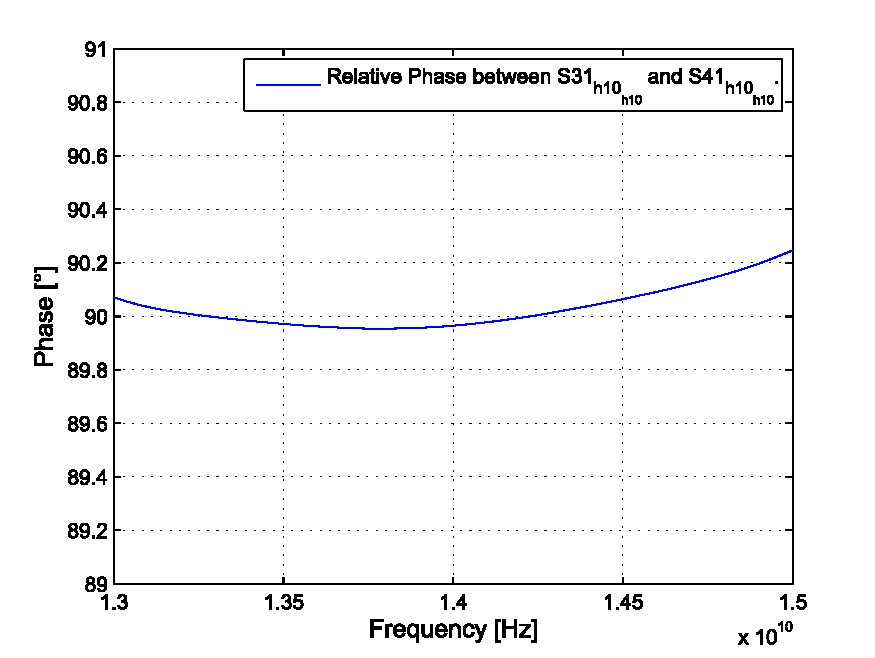
\includegraphics[width=7cm]{IQResults}
\caption{Caratteristica I/Q.}
\label{fig:Phase}
\end{minipage}
\hspace{0.1cm} % To get a little bit of space between the figures
\begin{minipage}[b]{0.5\linewidth}
\centering
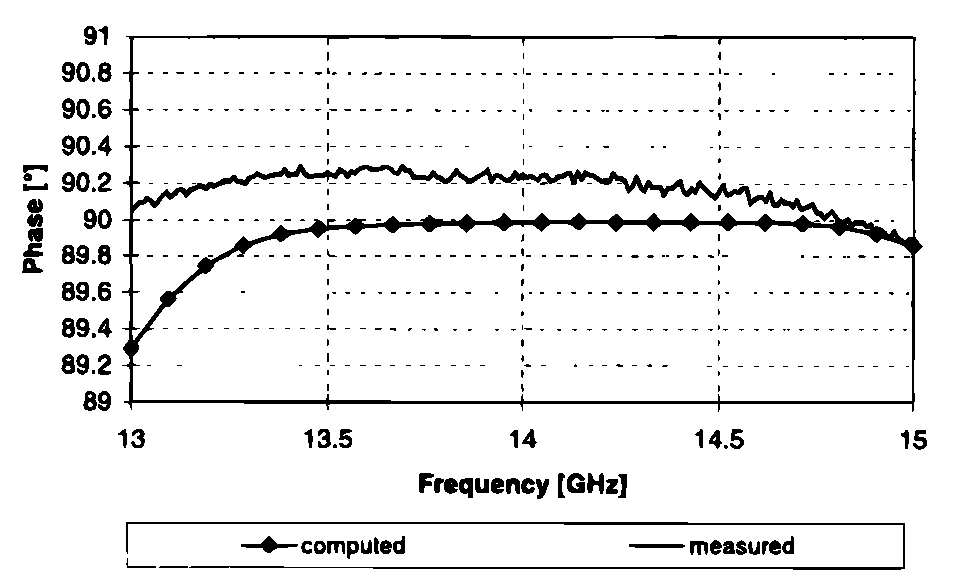
\includegraphics[width=7cm]{HildPaperPhase}
\caption{Caratteristica I/Q ottenuta da Hildebrand.}
\label{fig:PhaseH}
\end{minipage}
\end{figure}
\par Infine nelle figure \ref{fig:Phase} e \ref{fig:PhaseH} viene illustata la caratteristica in fase e quadratura dei segnali che fuoriescono dalle porte dirette e accoppiata. La fase relativa avvicina nettamente i 90 gradi entro i 6.5\% di banda di lavoro.
%%%%%%%%%%%%%%%%%%%%%%%%%%%%%%%%%%%%%%%%%%%%%%%%%%%%%%%%%%%%%%%%%%%%%%%%%%%%%%%% % CC
\section{Conclusione}

\par \`E stata presentata la tecnica del \textit{mode matching} in strutture guidanti a sezione rettangolare, delineando gli aspetti fondamentali per la realizzazione di un codice numerico. L'implementazione al calcolatore di questa tecnica \`e stata utilizzata per simulare in un primo momento una biforcazione nel piano H e poi l'accoppiatore direzionale di Hildebrand. Nel loro complesso i risultati ottenuti, a confronto per la prima simulazione con quelli ricavati da una simulazione della biforcazione con HFFS e per la seconda con quelli pubblicati da Hildebrand, hanno dimostrato la validit\`a dell'implementazione.

\par Le tipologie di discontinuit\`a strutturali che il codice realizzato permette di analizzare sono i gradini e quindi la cascata di gradini, e le giunzioni N a 1. Vi \`e un ulteriore tipo di giunzione, la giunzione a T, che sollecita un particolare interesse in quanto permetterebbe di estendere l'unico grado di libert\`a di propagazione del campo lungo $\mathbf{\hat{z}}$ delle precedenti strutture ai tre gradi di libert\`a del caso tridimensionale \cite{SieveArndt}.

\par L'alta efficienza computazionale del \textit{mode matching} offre la possibilit\`a di analizzare in tempi brevi e con adeguata accuratezza strutture guidanti altamente complesse quali filtri, accoppiatori e ben altri. Questa tecnica numerica rappresenta quindi un potente strumento nella progettazione e l'ottimizzazione di strutture guidanti.
%%%%%%%%%%%%%%%%%%%%%%%%%%%%%%%%%%%%%%%%%%%%%%%%%%%%%%%%%%%%%%%%%%%%%%%%%%%%%%%% % BIBLIOGRAFIA
\begin{thebibliography}{9}

\bibitem{CABalanis} C. A. Balanis, \emph{Advanced Engineering Electromagnetics}, New York: Wiley, 1989.

\bibitem{GGGentili} G. G. Gentili, \emph{Properties of TE-TM Mode-Matching Techniques}, IEEE Microwave and Guided Wave Letters, Vol. 39, No. 9, September 1991, pp. 1669-1673.

%\bibitem{TItoh} T. Itoh, \emph{Numerical Techniques for Microwave and Millimeter-Wave Passive Structures}, New York: Wiley, 1989, pp. 592�621.
% altre tecniche di proiezione

\bibitem{SSelleri} S. Selleri, \emph{How to Condense GSMs}, IEEE Transactions.

\bibitem{LTHildebrand} L. T. Hildebrand, \emph{Results for a Simple Compact Narrow-Wall Directional Coupler}, IEEE Microwave and Guided Wave Letters, Vol. 10, No. 6, June 2000, pp. 231-232.

\bibitem{HJRiblet} H. J. Riblet, \emph{The Short-Slot Hybrid Junction}, Proceedings of the Institute of Radio Engineers, Vol. 40, No. 2, February 1952, pp. 180-184.

\bibitem{SteerTrew} M. B. Steer, R. J. Trew, \emph{``Microwave Device'', The Electrical Engineering Handbook} Ed. Richard C. Dorf, Boca Raton: CRC Press LLC, 2000.

\bibitem{SieveArndt} T. Sieverding, F. Arndt, \emph{Field Theoretic CAD of Open or Aperture Matched T-Junction Coupled Rectangular Waveguide Structures}, IEEE Microwave and Guided Wave Letters, Vol. 40, No. 2, February 1992, pp. 353-362.

\end{thebibliography}

\end{document}
